\section{Results}
\label{sec:results}

\paragraph{Setup}
One person recorded 8 egocentric videos of household chores (counter wiping, cloth folding, bed making, cable wrapping), about 10 minutes each. TransNetV2~\cite{transnetv2} split them into 116 clips of at most 15~s at 4~fps and $854\times480$, about 30 minutes in total. All runs used one A100 80~GB. Per clip, reasoning took 130~s, a Transfer render 20~min and a Predict2 render 3.5~min; GPT-4o mini for all 116 clips cost about 0.12 USD. We ran reasoning on all 116 clips and rendered 64 Transfer variants of 10 source clips plus two Predict2 clips; at these rates the 116 clips could become $116\times72 = 8{,}352$ variants at about 2{,}800 A100-hours. No policy was trained on the output.

\subsection{Appearance Variation}
Fig.~\ref{fig:teaser} is the running example under the blue-countertop prompt. The counter is blue, hand pose and bucket geometry are preserved frame for frame, and the motion is the source motion. Every unintended change is also easy to see: the rags became blue cloth, the bucket grey-blue, the wall beige, and a ceiling fixture appeared, although the prompt named the bucket, towels and lighting as preserved. Fig.~\ref{fig:more}a,b shows the cloth-folding clip, where the prompt asked for a cobalt blanket on the left of the bed and the render turned nearly every surface blue. Where the counter clip leaks at the edges of the target, a frame with many textures fails almost completely. Fig.~\ref{fig:more}c,d show a blue-desk prompt whose color spreads onto the shelf objects and the cable, and a navy-rug prompt that returned the right bedspread with smeared surfaces and a warped hand, the shape-collapse failure of Table~\ref{tab:weights}.

\begin{figure}[t]
\centering
\begin{subfigure}[t]{0.30\linewidth}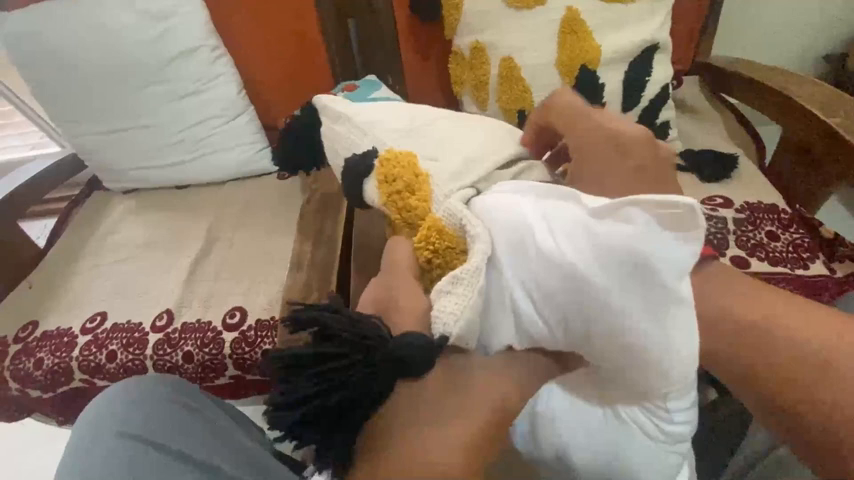
\includegraphics[width=\linewidth]{s14_old.png}\caption{cloth folding, source}\end{subfigure}\hspace{2mm}
\begin{subfigure}[t]{0.30\linewidth}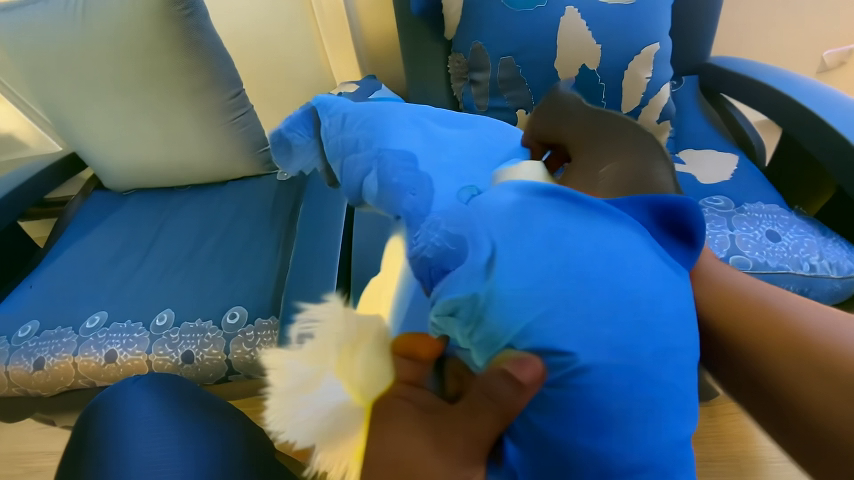
\includegraphics[width=\linewidth]{s14_new.png}\caption{cobalt blanket prompt}\end{subfigure}\\[1.5mm]
\begin{subfigure}[t]{0.105\linewidth}\centering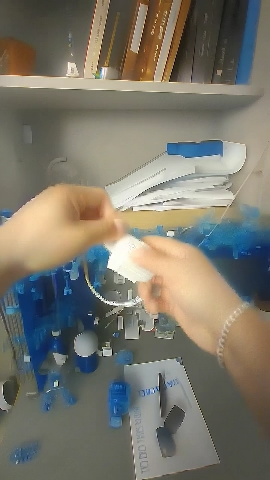
\includegraphics[height=1.6cm]{s16_left.png}\caption{}\end{subfigure}\hfill
\begin{subfigure}[t]{0.29\linewidth}\centering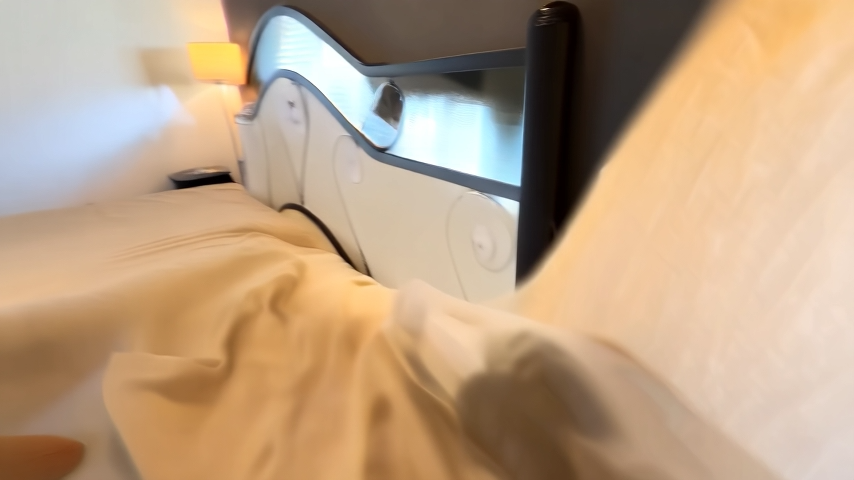
\includegraphics[height=1.6cm]{s16_middle.png}\caption{}\end{subfigure}\hfill
\begin{subfigure}[t]{0.29\linewidth}\centering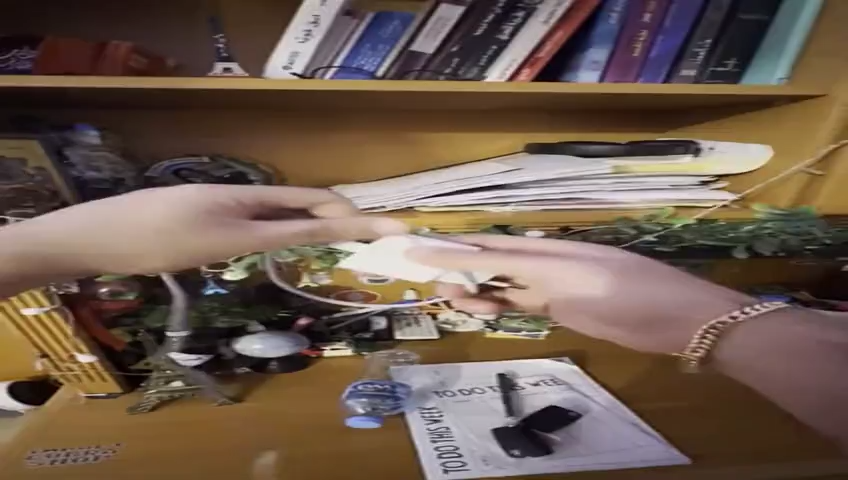
\includegraphics[height=1.6cm]{s15_generated.png}\caption{}\end{subfigure}\hfill
\begin{subfigure}[t]{0.29\linewidth}\centering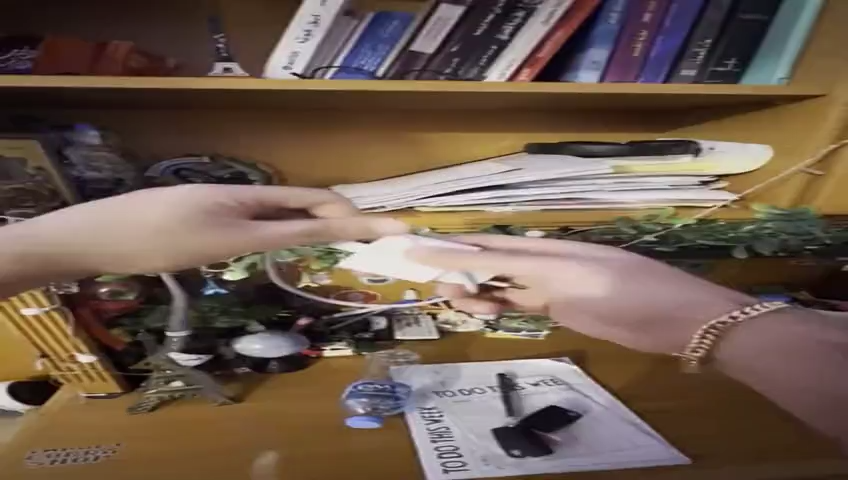
\includegraphics[height=1.6cm]{s16_right.png}\caption{}\end{subfigure}
\caption{Where the renders fail. (a, b) The prompt targeted one blanket; the render recolored cushions, chair and cloth. (c) Blue desk: color spreads onto the shelf objects and cable. (d) Navy-rug prompt: the bedspread is right, surfaces smear and the hand warps. (e, f) Predict2 cable-wrapping and paper-rotation prompts: nothing moves.}
\label{fig:more}
\end{figure}

\subsection{Measuring Leakage}
\label{sec:leakage}
To put a number on the unintended change we compare source and variant frame by frame in CIELAB and split the per-pixel CIE76 distance $\Delta E$ by the tracked mask $M$; a $\Delta E$ of 10 is unmistakable to a viewer. Table~\ref{tab:leakage} gives the result for the counter clip, the one render with a usable tracked mask. The target moved by a mean $\Delta E$ of 75, so the recolor worked. The protected region moved by 35, 95\% of its pixels moved by more than 10, and the chroma-only distance shows the change is color rather than exposure. The seg control and the prompt's preservation clause were the two soft mechanisms for containment, and neither was sufficient.

\begin{table}[t]
\centering
\caption{Masked color difference for the counter-wiping variant over 60 frames; each region covers about half the frame. The protected region changes by almost half as much as the target, and nearly all of it changes visibly.}
\label{tab:leakage}
\small
\begin{tabular}{@{}lrr@{}}
\toprule
 & Target ($M$) & Protected ($\bar M$) \\
\midrule
Mean $\Delta E$ & 75.5 & 34.8 \\
Mean chroma-only $\Delta E$ ($a$, $b$ channels) & 68.2 & 24.2 \\
Pixels with $\Delta E > 10$ (\%) & -- & 94.5 \\
Pixels with $\Delta E > 20$ (\%) & -- & 65.3 \\
\bottomrule
\end{tabular}
\end{table}

\subsection{Action-Level Variation}
\label{sec:action}
Two action variations from the ontology were run through Predict2 (35 steps, $848\times480$, 93 frames at 16~fps): winding a charger cable around its block with the block held fixed, and a sheet of paper rotating 90 degrees while the objects on it stay put. In both renders the forecast reproduces the conditioning scene and the cable and paper do not move (Fig.~\ref{fig:more}e,f). The model held the scene stable, a kind of success for a world model, and did not perform the action, the only thing we asked of it.
